\chapter{Lezione 7 - Workflow - Flusso lavorativo}

Benvenuti a tutti a questa lezione sul flusso lavorativo, workflow.
Gli argomenti che tratteremo in questa lezione sono due definizioni di flusso di lavoro, vedremo le caratteristiche di un sistema per la gestione automatica dei flussi di lavoro e analizzeremo l'architettura di un sistema per la gestione dei flussi di lavoro presentata dalla workflow management coalition.

Argomenti trattati:

\FloatBarrier
\begin{figure}[H]
  \centering
  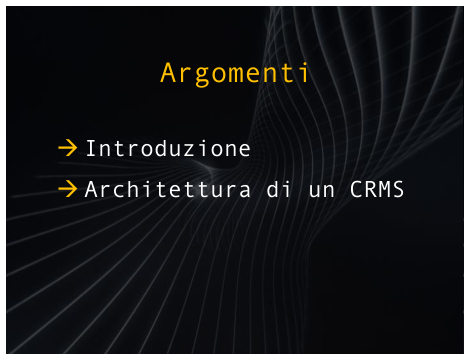
\includegraphics[width=0.50\textwidth,
                    trim=40 100 40 60, % L B R T
                    clip]
                    {images/Lez08_p01_fig_02}
  % \caption{Sommario}
  % \label{fig:Lez15_p06_fig_02}
\end{figure}
\FloatBarrier
\noindent

